

%*************************************************************************
% Chapter Quote
\begin{savequote}[50mm]
‘‘Equipped with his five senses, man explores the universe around him and 
calls the adventure Science’’
\qauthor{Edwin Hubble}
\end{savequote}
%*************************************************************************


\chapter{Introduction}
\label{cha:Introduction}

 
%*************************************************************************
% Introduction to the Introduction

‘‘What is our place in the cosmos?’’ This is one of the more simple and 
trans\-cendental question of the human beings, and powered by our innate 
curiosity has led to a current relatively understandable picture of our 
Universe. In fact, the astronomy and specifically the cosmology and large
scale structure formation can be only considered as a scientific rigorous
disciplines after the seventeenth century.

\

Almost in every scientific discipline a significant theoretical advance is 
accompanied of a technical improvement of its own instruments, it is for this 
reason that at the beginning of the seventeenth century Johannes Kepler could
establish his three well-known empirical laws of the planetary movements 
based on the very precise data of astronomical bodies computed for Tycho Brahe. 
This event was very remarkable in the astronomy history due to was the first
of many strikes against the well established anthropomorphic notion of the 
cosmos. Although the Kepler laws constituted the most crucial test to the Nicolaus 
Copernicus heliocentric model, it was only until 1685 when Isaac Newton 
formulated the law of universal gravitation (from which can be derived all 
the Kepler laws) when the astronomers could have a enough powerful tools to
begin a depth and serious discussion about the real nature of our universe on 
scales bigger than the solar system, and thus inaugurating the \textit{sciences 
of gravity} \cite{longair2008}

\

After the establishment of the universal gravitation, the next significative 
theo\-retical achievement in this area came in the centuries eighteenth and 
nineteenth with the development of classical mechanics, as the Hamiltonian 
and Lagrangian formalism, and powerful numerical tools. All this achievements 
impulse the study of key topics as the many body problem, allowing a depth 
understanding of the dynamic of complex gravitational system, as planetary
system, star clusters, galaxies, etc. 

\

Parallel to previous theoretical advances, in the observational side was 
beginning to arise the idea of \textit{island universe}, from which will 
evolve the concept of galaxy. This was powered by the development of the 
telescope, allowing besides to understand that the galaxy is only a large 
collection of stars like our sun. It was very remarkable the pioneer work of 
William Herschel, who tried to make a map of our galaxy determining distances 
with the assumption that stars have the same intrinsic luminosity and the 
inverse square law for the intensity decay (see figure \ref{fig:HerschelModel}). 
Although his results were very imprecise due to the incorrect assumption on 
which were based, the importance of his work lies in the recognition of a 
structure (disk-like) for our galaxy. 

%.........................................................................
%Herschel Model of Our Galaxy
\begin{figure}[htbp]
	\centering
	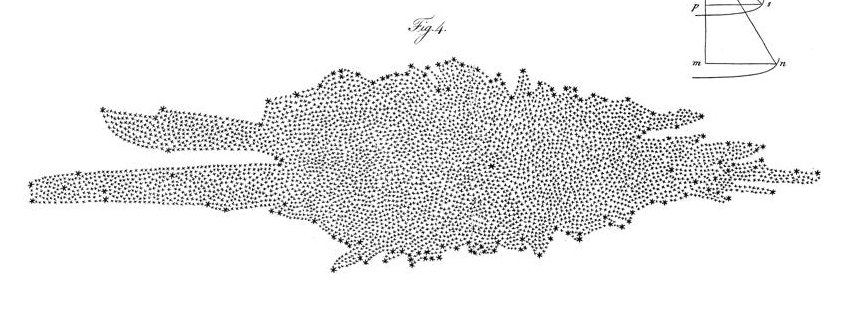
\includegraphics[width=1.0\textwidth]{./figures/1_introduction/Herschel_Model.png}
	
	\caption{\small{William Herschel's model of our galaxy based upon star 
	counts and the equal luminosity assumption.\cite{Herschel1785}}}
	
	\label{fig:HerschelModel}
\end{figure}
%.........................................................................

Another important observational question that was emerging in that epoch is 
about the existence of \textit{island universes} like ours. It was already 
well known the existence of extended objects that do not fit to definition of
stars or planets, as nebulae, planetary disks and galaxies. Even William
Herschel and his son John Herschel contributed with the realization of an
large (for the epoch) catalogue of extended bodies

 but their real 
nature was a complete mystery, even if they are objects inside our galaxy 
or completely independent systems.






%*************************************************************************
%*************************************************************************
%The current cosmology picture
\section{The Current Cosmology Picture}
\label{sec:TheCurrentCosmologyPicture}


	%---------------------------------------------------------------------
	%First stage of our universe
	\subsection{First Stage of Our Universe}
	\label{subsec:FirstStageOfOurUniverse}
	%---------------------------------------------------------------------


	%---------------------------------------------------------------------
	%Nonlinear epoch
	\subsection{Nonlinear Epoch}
	\label{subsec:NonlinearEpoch}
	%---------------------------------------------------------------------


	%---------------------------------------------------------------------
	%Our local neighborhood, the Local Group
	\subsection{Our Local Neighborhood, the Local Group}
	\label{subsec:OurLocalNeighborhood}
	%---------------------------------------------------------------------


%*************************************************************************
%*************************************************************************
%Numerical simulations
\section{Numerical Simulations}
\label{sec:NumericalSimulations}


	%---------------------------------------------------------------------
	%N-body simulations
	\subsection{N-body Simulations}
	\label{subsec:N-bodySimulations}
	%---------------------------------------------------------------------
	
	
	%---------------------------------------------------------------------
	%The comological environment
	\subsection{The Cosmological Environment}
	\label{subsec:TheCosmologicalEnvironment}
	%---------------------------------------------------------------------
	
	
	%---------------------------------------------------------------------
	%Concordance with real world
	\subsection{Concordance with Real World}
	\label{subsec:ConcordanceWithRealWorld}
	%---------------------------------------------------------------------
	
	

%*************************************************************************
%*************************************************************************
%Cosmological observations
\section{Cosmological Observations}
\label{sec:CosmologicalObservations}


	%---------------------------------------------------------------------
	%COBE
	\subsection{COBE}
	\label{subsec:COBE}
	%---------------------------------------------------------------------
	
	
	%---------------------------------------------------------------------
	%WMAP
	\subsection{WMAP}
	\label{subsec:WMAP}
	%---------------------------------------------------------------------
	
	
	%---------------------------------------------------------------------
	%Planck
	\subsection{Planck}
	\label{subsec:Planck}
	%---------------------------------------------------------------------
%*************************************************************************

